\documentclass[6pt]{../../shared/AiTex}
\usepackage{csvsimple}
\usepackage{pdflscape}

\title{Memoria entrega 4}
\author{A.L.K.}
\date{Febrero 2024}

\begin{document}
%\datos{facultad}{universidad}{grado}{asignatura}{subtitulo}{autor}{curso}
\datos{Informática}{Universidad Complutense de Madrid}{Ingeniería informática}{Aprendizaje Automatico y Big Data}{Entrega 6: diseño de redes neuronales}{Alejandro Barrachina Argudo}{2023-2024}
% \portadaApuntes
% \pagestyle{empty}
% \tableofcontents
% \pagestyle{empty}
\justify

\begin{center}

    {\huge \textbf{\underline{\subtitulo}}} \\
    { \lesson - \autor}

\end{center}


\section*{Introducción}

En este documento se explicará el código del entregable 6 y el proceso de diseño de redes neuronales.

Para esta práctica se usarán los siguientes \textit{imports} vistos en la figura \ref{fig:imports}. Parte del código se reutiliza de la práctica anterior.
\begin{figure}[H]
    \centering
    \lstinputlisting[firstline=1,lastline=9, style=custompython]{../design.py}
    \caption{Código de las bibliotecas usadas}
    \label{fig:imports}
\end{figure}

También usaremos una serie de constantes para todo el programa (figura \ref{fig:constants}).

\begin{figure}[H]
    \centering
    \lstinputlisting[firstline=11,lastline=17, style=custompython]{../design.py}
    \caption{Constantes del programa}
    \label{fig:constants}
\end{figure}

El \textit{dataset} para esta práctica lo generamos aleatoriamente con la función \textit{gen\_data} (figura \ref{fig:gen_data}). El dataset se compone de una linea de datos ``ideales'' y datos con ruido para comprobar la eficacia de la red neuronal.

Para dibujar estos datos usaremos la función \textit{plot\_dataset} (figura \ref{fig:plot_dataset}).

\begin{figure}[H]
    \centering
    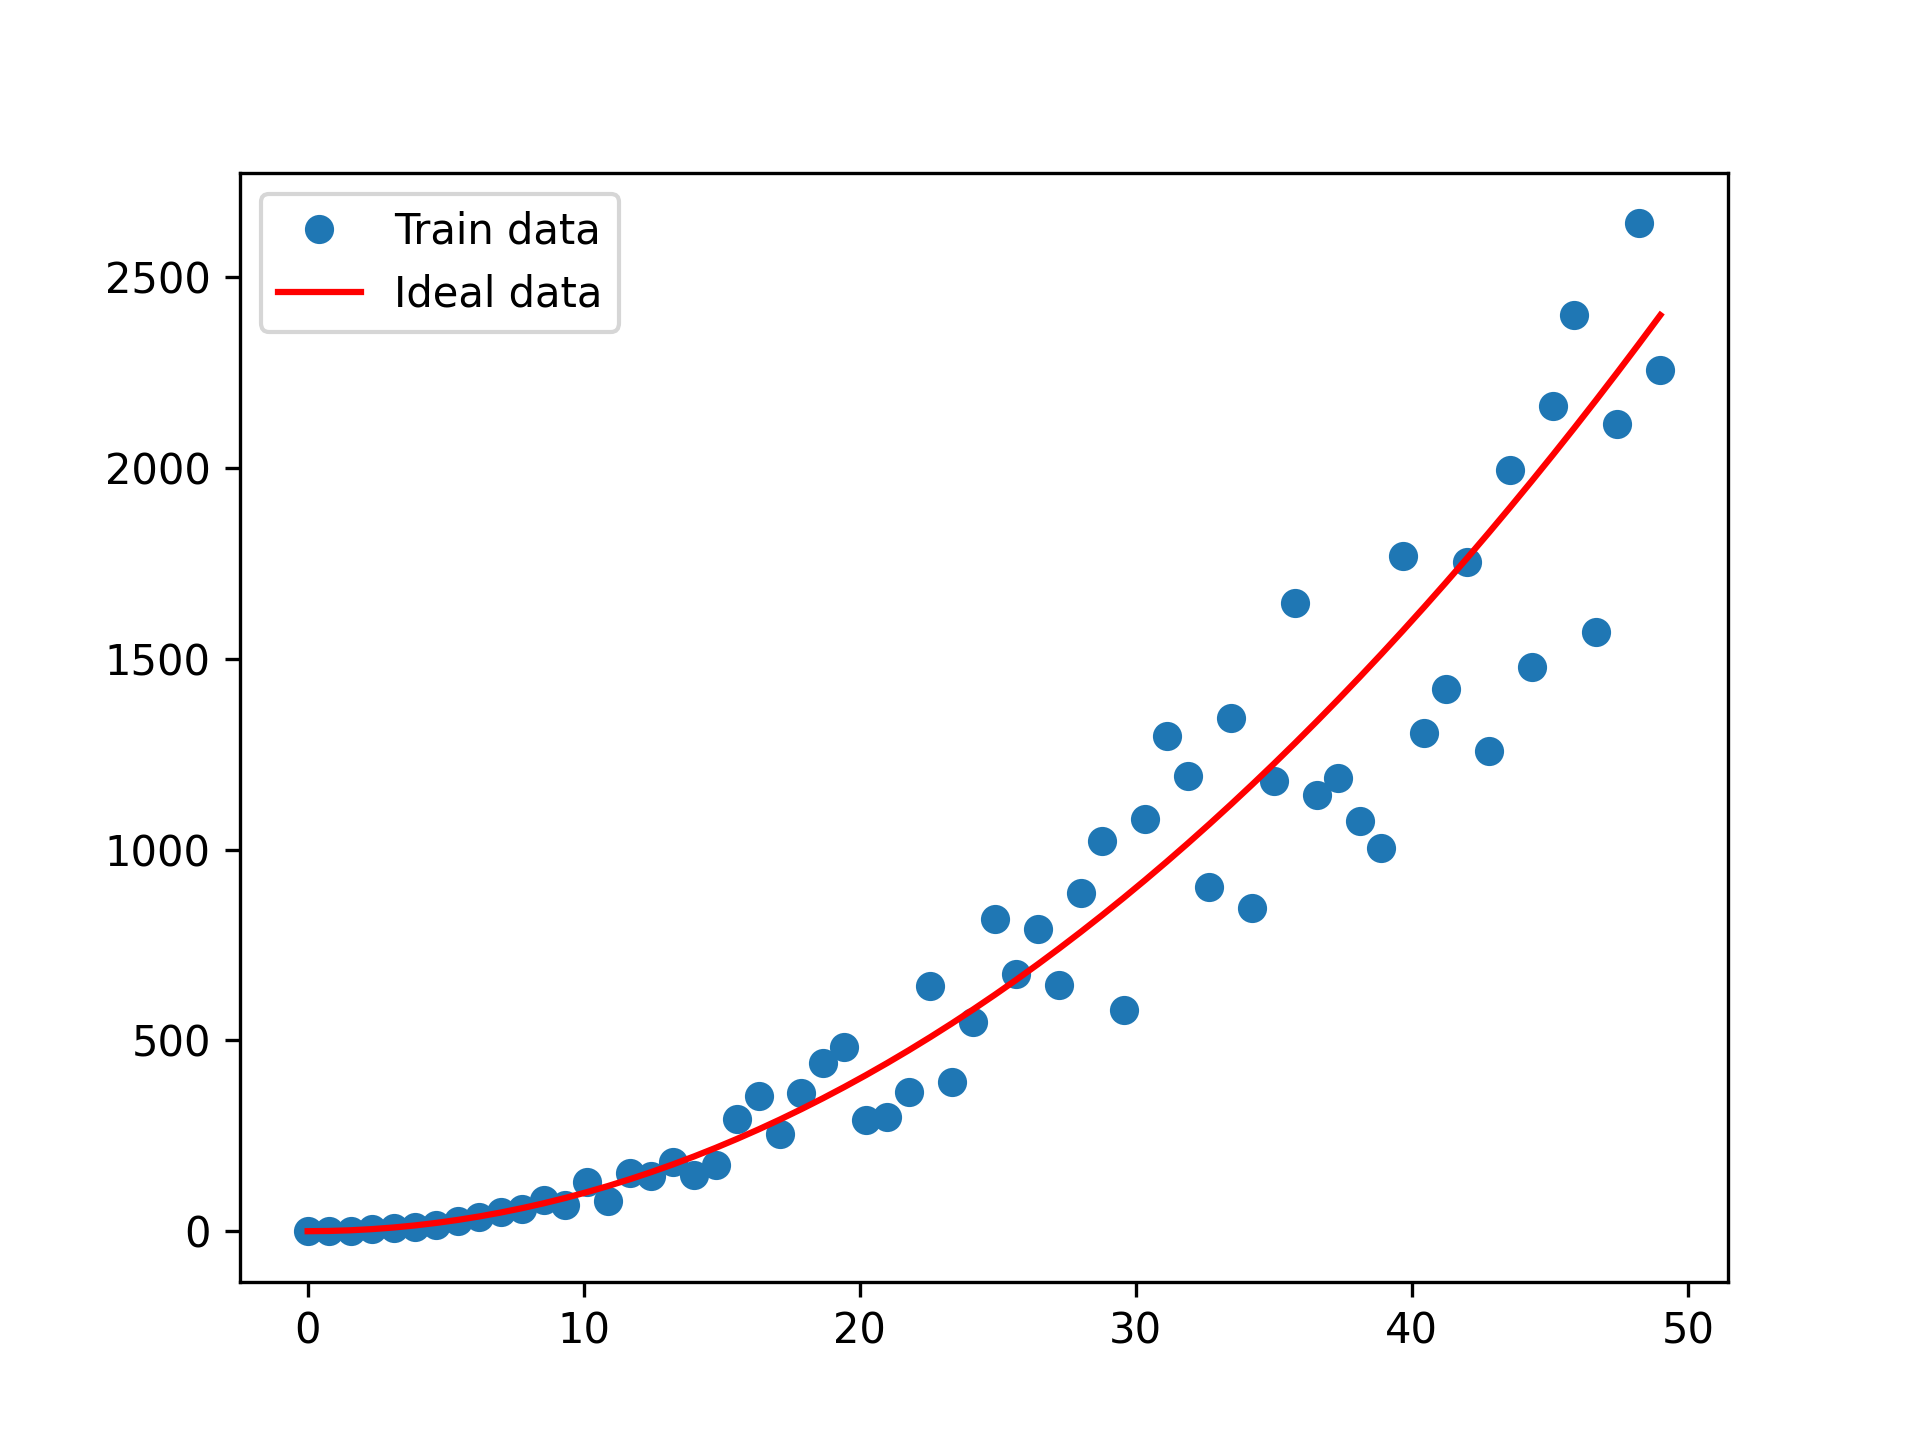
\includegraphics[width=0.5\textwidth]{./images/dataset.png}
    \caption{Ejemplo de los dígitos del \textit{dataset}}
    \label{fig:digitos}
\end{figure}

\begin{figure}[H]
    \centering
    \lstinputlisting[firstline=92,lastline=110, style=custompython]{../design.py}
    \caption{Función \textit{gen\_data}}
    \label{fig:gen_data}
\end{figure}

\begin{figure}[H]
    \centering
    \lstinputlisting[firstline=20,lastline=34, style=custompython]{../design.py}
    \caption{Función \textit{plot\_dataset}}
    \label{fig:plot_dataset}
\end{figure}

\section{Sobreajuste a los ejemplos de entrenamiento}

En este apartado vamos a analizar lo que ocurre si tienes pocos datos de test, haciendo así que el problema se amolde solo a los datos de entrenamiento y no consiga generalizar.

Para ello usaremos la función \textit{overfitting} (figura \ref{fig:overfitting}). Dentro de esta función primero hacemos una separación de los datos para dejar un porcentaje del 67\% a los datos de entrenamiento y un 33\% a los datos de entrenamiento. Seguido esto, utilizamos las funciones \textit{train}(\ref{fig:train}) para entrenar el modelo lineal y \textit{test}(\ref{fig:test}) para sacar los costes (función \textit{cost}, figura \ref{fig:cost}) de ambos conjuntos de datos. La figura \ref{fig:overfitting_plot} nos muestra en gráfica el sobreajuste producido por esta función. Este gráfico se genera con la función \textit{plot\_linear\_data} (figura \ref{fig:plot_linear_data}).

\begin{figure}[H]
    \centering
    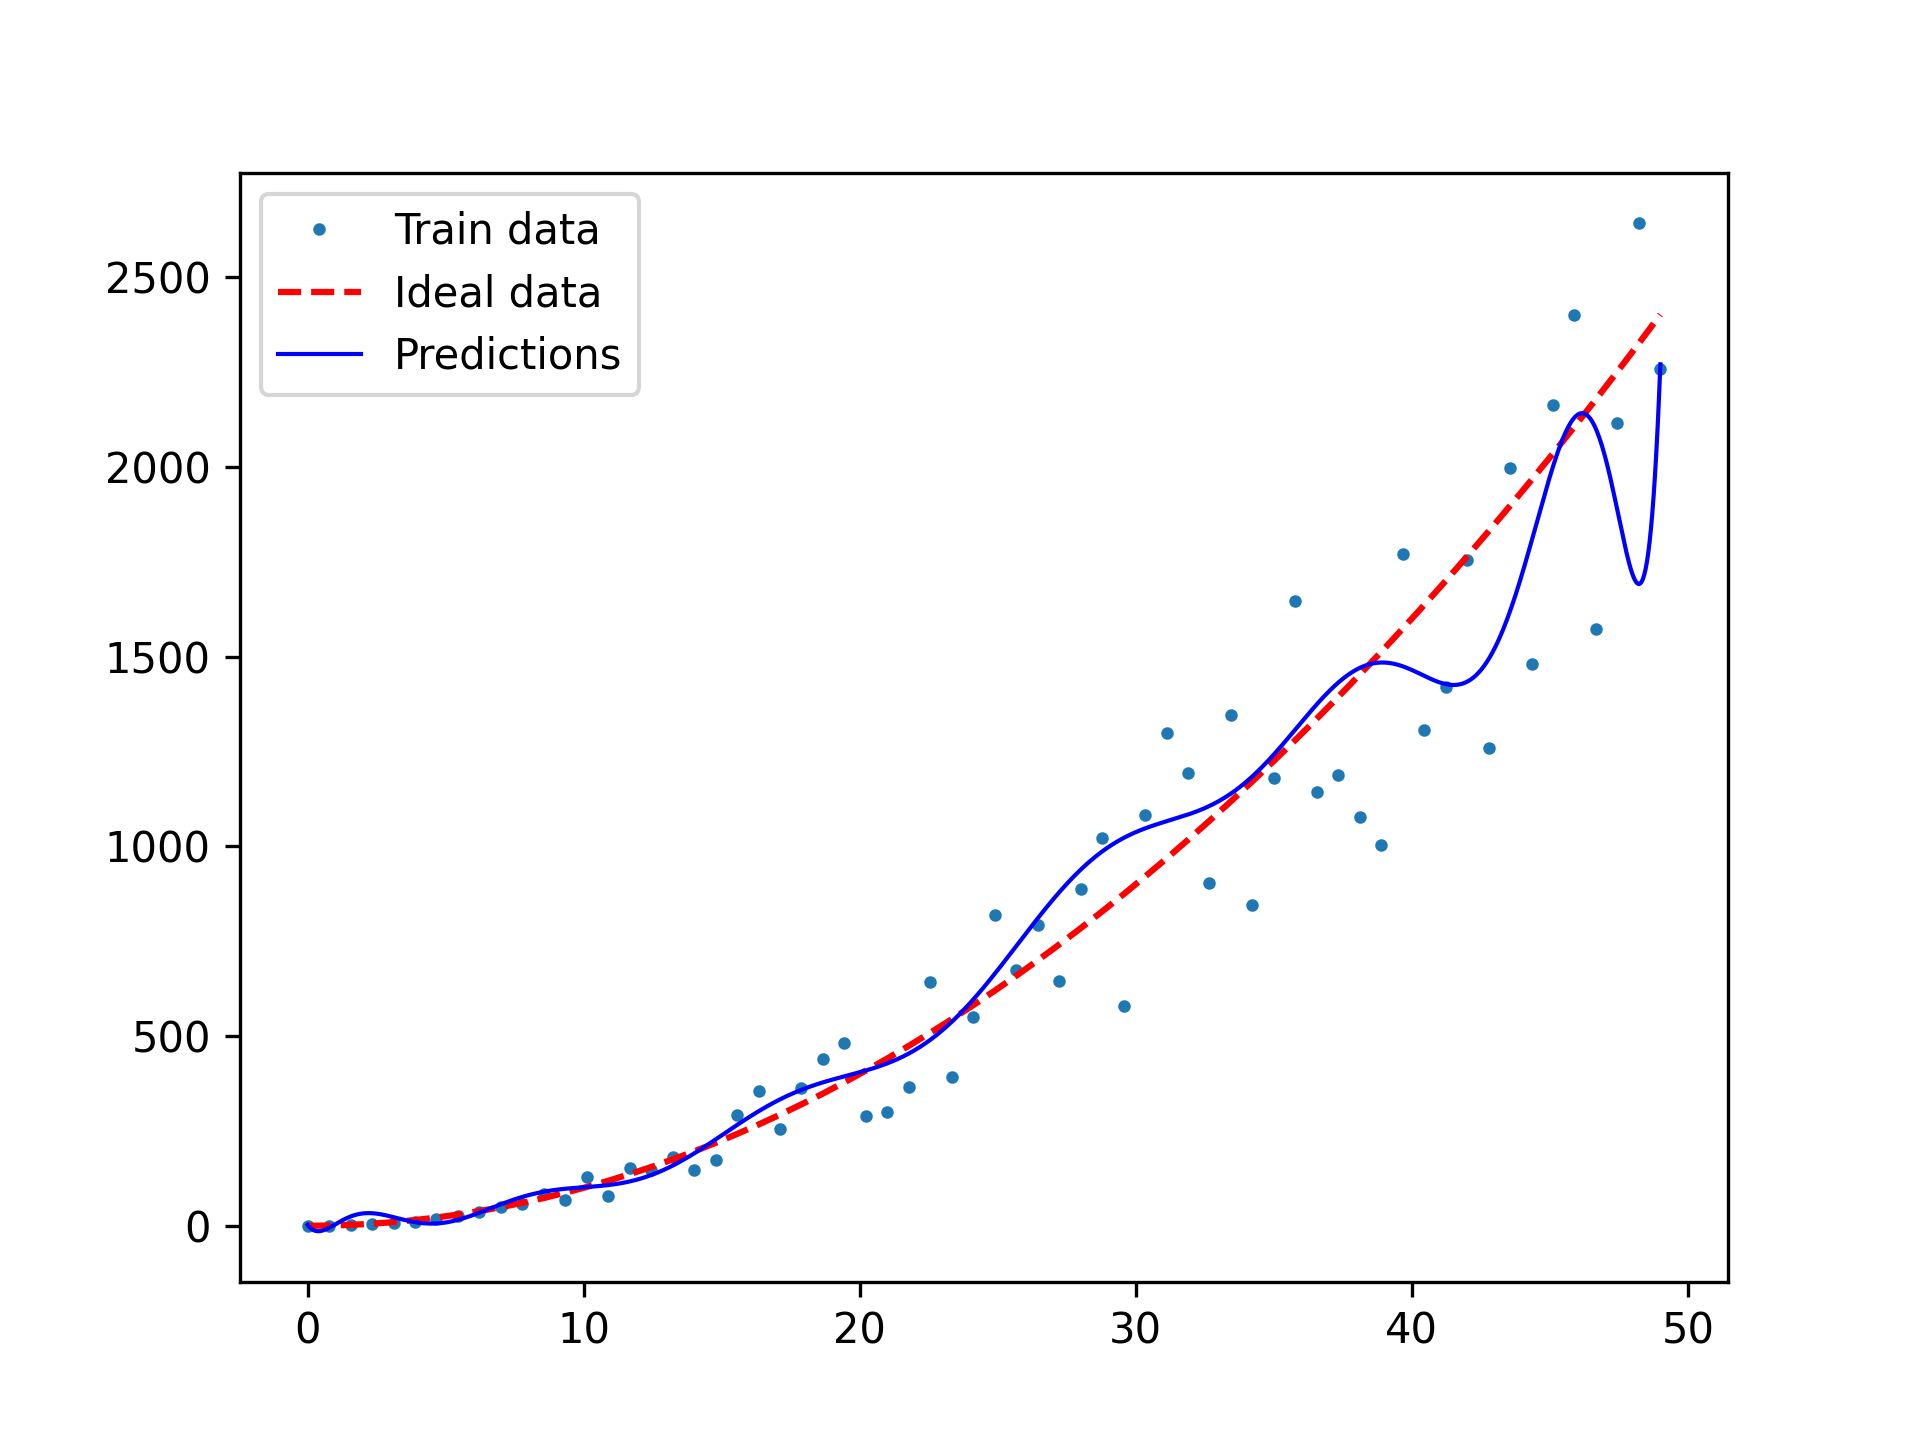
\includegraphics[width=0.5\textwidth]{./images/overfitting.png}
    \caption{Gráfica del sobreajuste}
    \label{fig:overfitting_plot}
\end{figure}


\begin{figure}[H]
    \centering
    \lstinputlisting[firstline=196,lastline=219, style=custompython]{../design.py}
    \caption{Función \textit{overfitting}}
    \label{fig:overfitting}
\end{figure}

\begin{figure}[H]
    \centering
    \lstinputlisting[firstline=126,lastline=144, style=custompython]{../design.py}
    \caption{Función \textit{train}}
    \label{fig:train}
\end{figure}

\begin{figure}[H]
    \centering
    \lstinputlisting[firstline=169,lastline=193, style=custompython]{../design.py}
    \caption{Función \textit{test}}
    \label{fig:test}
\end{figure}

\begin{figure}[H]
    \centering
    \lstinputlisting[firstline=113,lastline=123, style=custompython]{../design.py}
    \caption{Función \textit{cost}}
    \label{fig:cost}
\end{figure}

\begin{figure}[H]
    \centering
    \lstinputlisting[firstline=37,lastline=55, style=custompython]{../design.py}
    \caption{Función \textit{plot\_linear\_data}}
    \label{fig:plot_linear_data}
\end{figure}

\section{Elección del grado del polinomio usando un conjunto de validación}

En este apartado vamos a escoger el grado del polinomio basándonos en el menor coste de validación de grados entre 1 y 10. Primero dividimos los datos en 60\% de entrenamiento, 20\% de validación y 20\% de test. Entrenamos el modelo con las funciones del apartado anterior (\ref{fig:train}, \ref{fig:test}) y escogemos el grado que menos coste de validación nos de.

La función que lleva todo este proceso es \textit{seleccion\_grado} (figura \ref{fig:seleccion_grado}). La figura \ref{fig:seleccion_grado_plot} nos muestra en la comparativa entre el modelo del grado escogido y la recta ideal. El grado escogido es 2.

\begin{figure}[H]
    \centering
    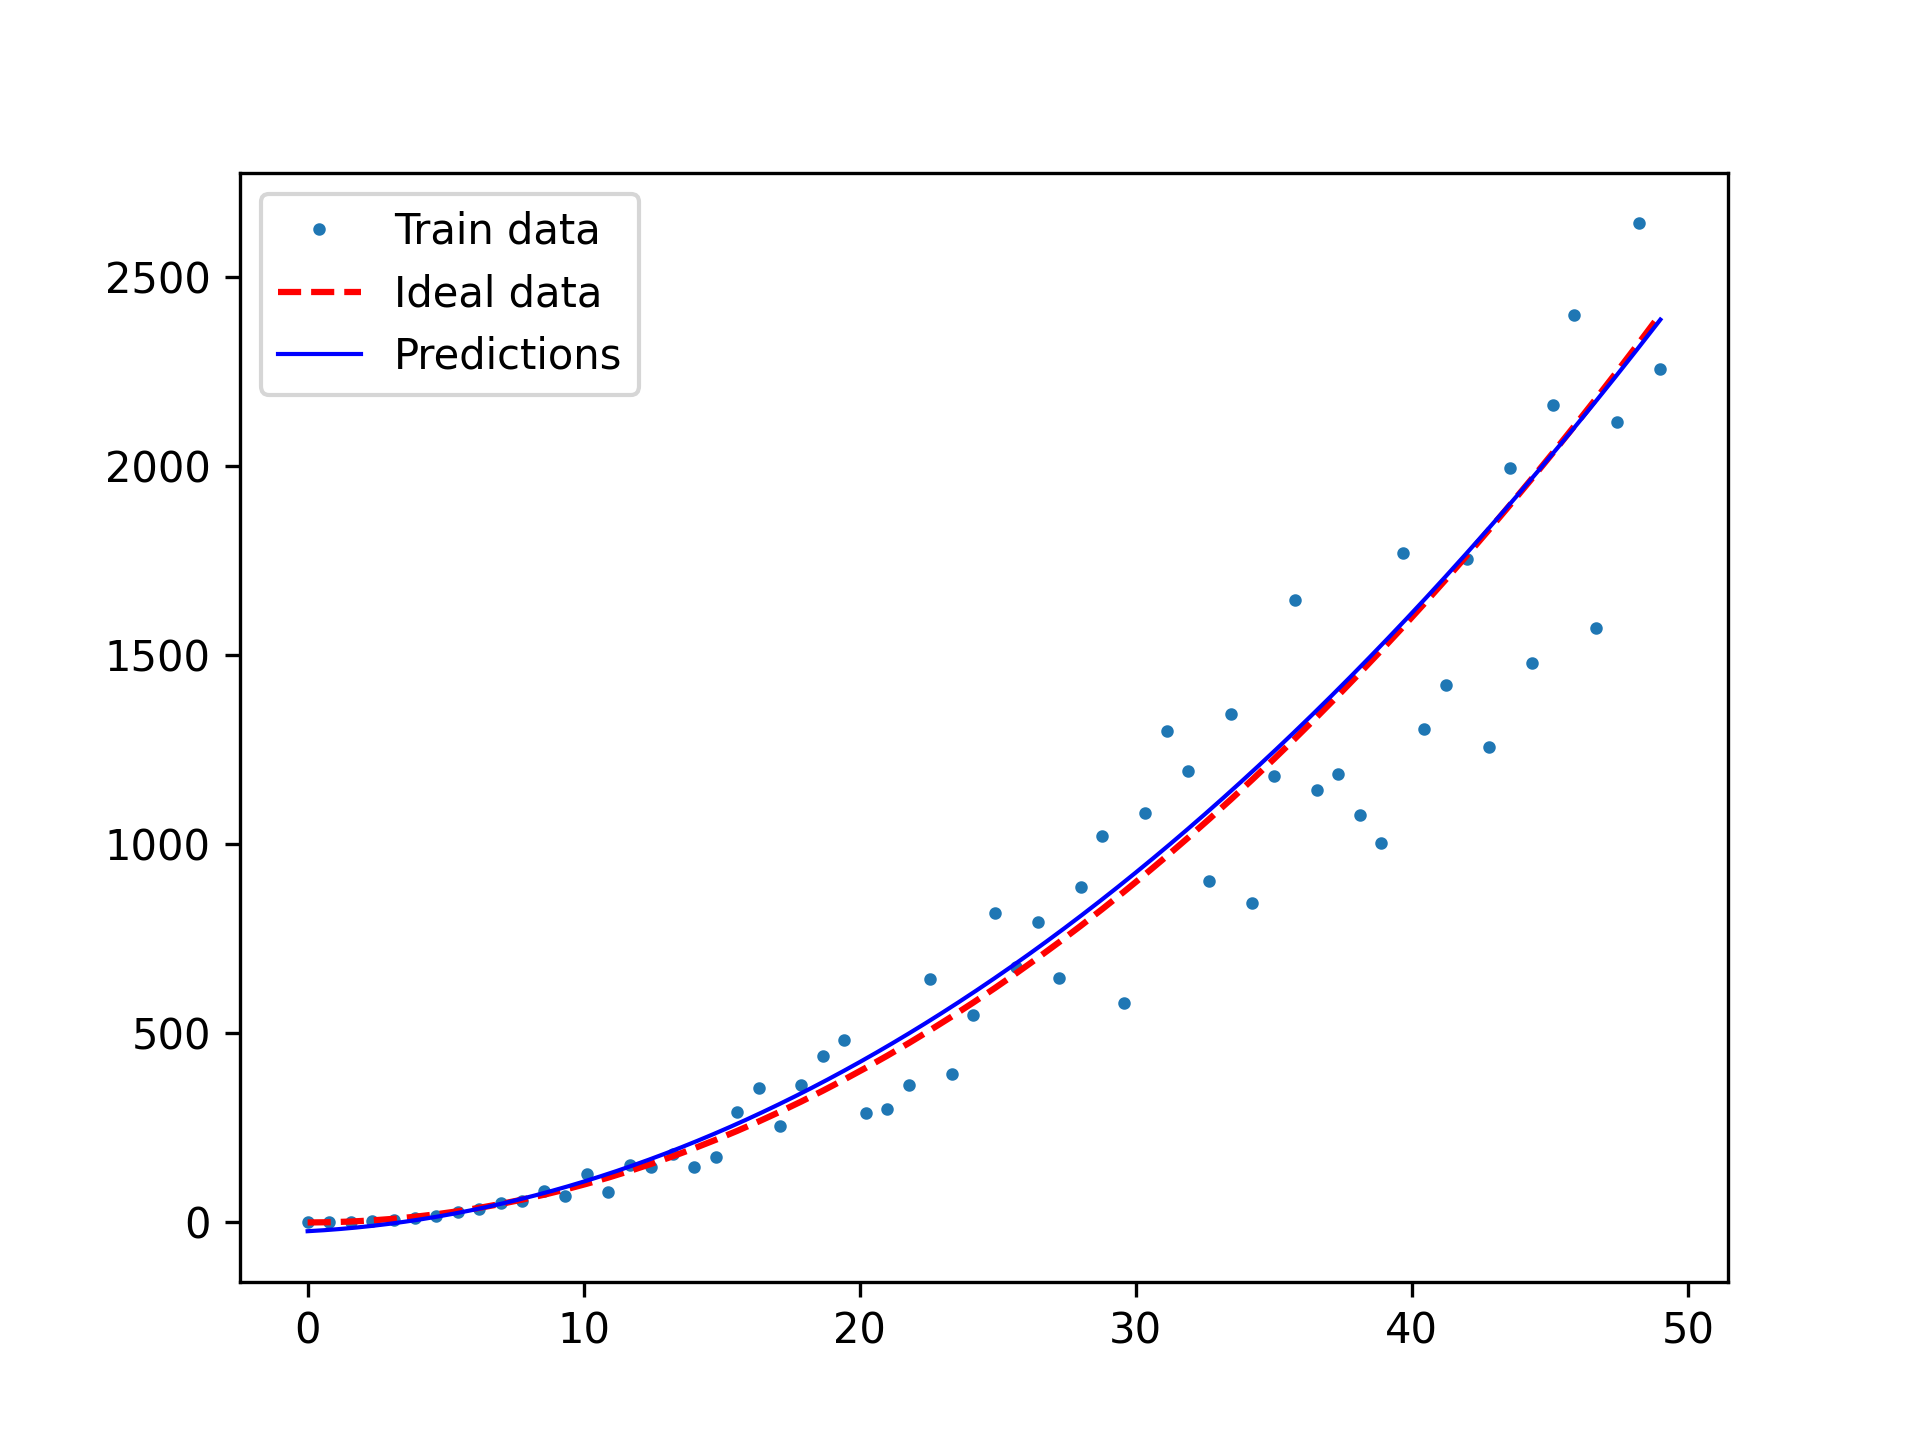
\includegraphics[width=0.5\textwidth]{./images/grado.png}
    \caption{Gráfica de la selección del grado}
    \label{fig:seleccion_grado_plot}
\end{figure}

\begin{figure}[H]
    \centering
    \lstinputlisting[firstline=222,lastline=261, style=custompython]{../design.py}
    \caption{Función \textit{seleccion\_grado}}
    \label{fig:seleccion_grado}
\end{figure}

\section{Elección del parámetro $\lambda$}

Como en este apartado usamos regularización, incluimos la funcion \textit{train\_reg} (figura \ref{fig:train_reg}) para entrenar el modelo con regularización, la función de test se mantiene igual. La función \textit{seleccion\_lambda} (figura \ref{fig:seleccion_lambda}) nos ayudará a escoger el mejor $\lambda$ entre [1e-6, 1e-5, 1e-4, 1e-3, 1e-2, 1e-1, 1, 10, 100, 300, 600, 900]. La figura \ref{fig:seleccion_lambda_plot} nos muestra la comparativa entre el modelo con el $\lambda$ escogido y la recta ideal. El $\lambda$ escogido es 10.

\begin{figure}[H]
    \centering
    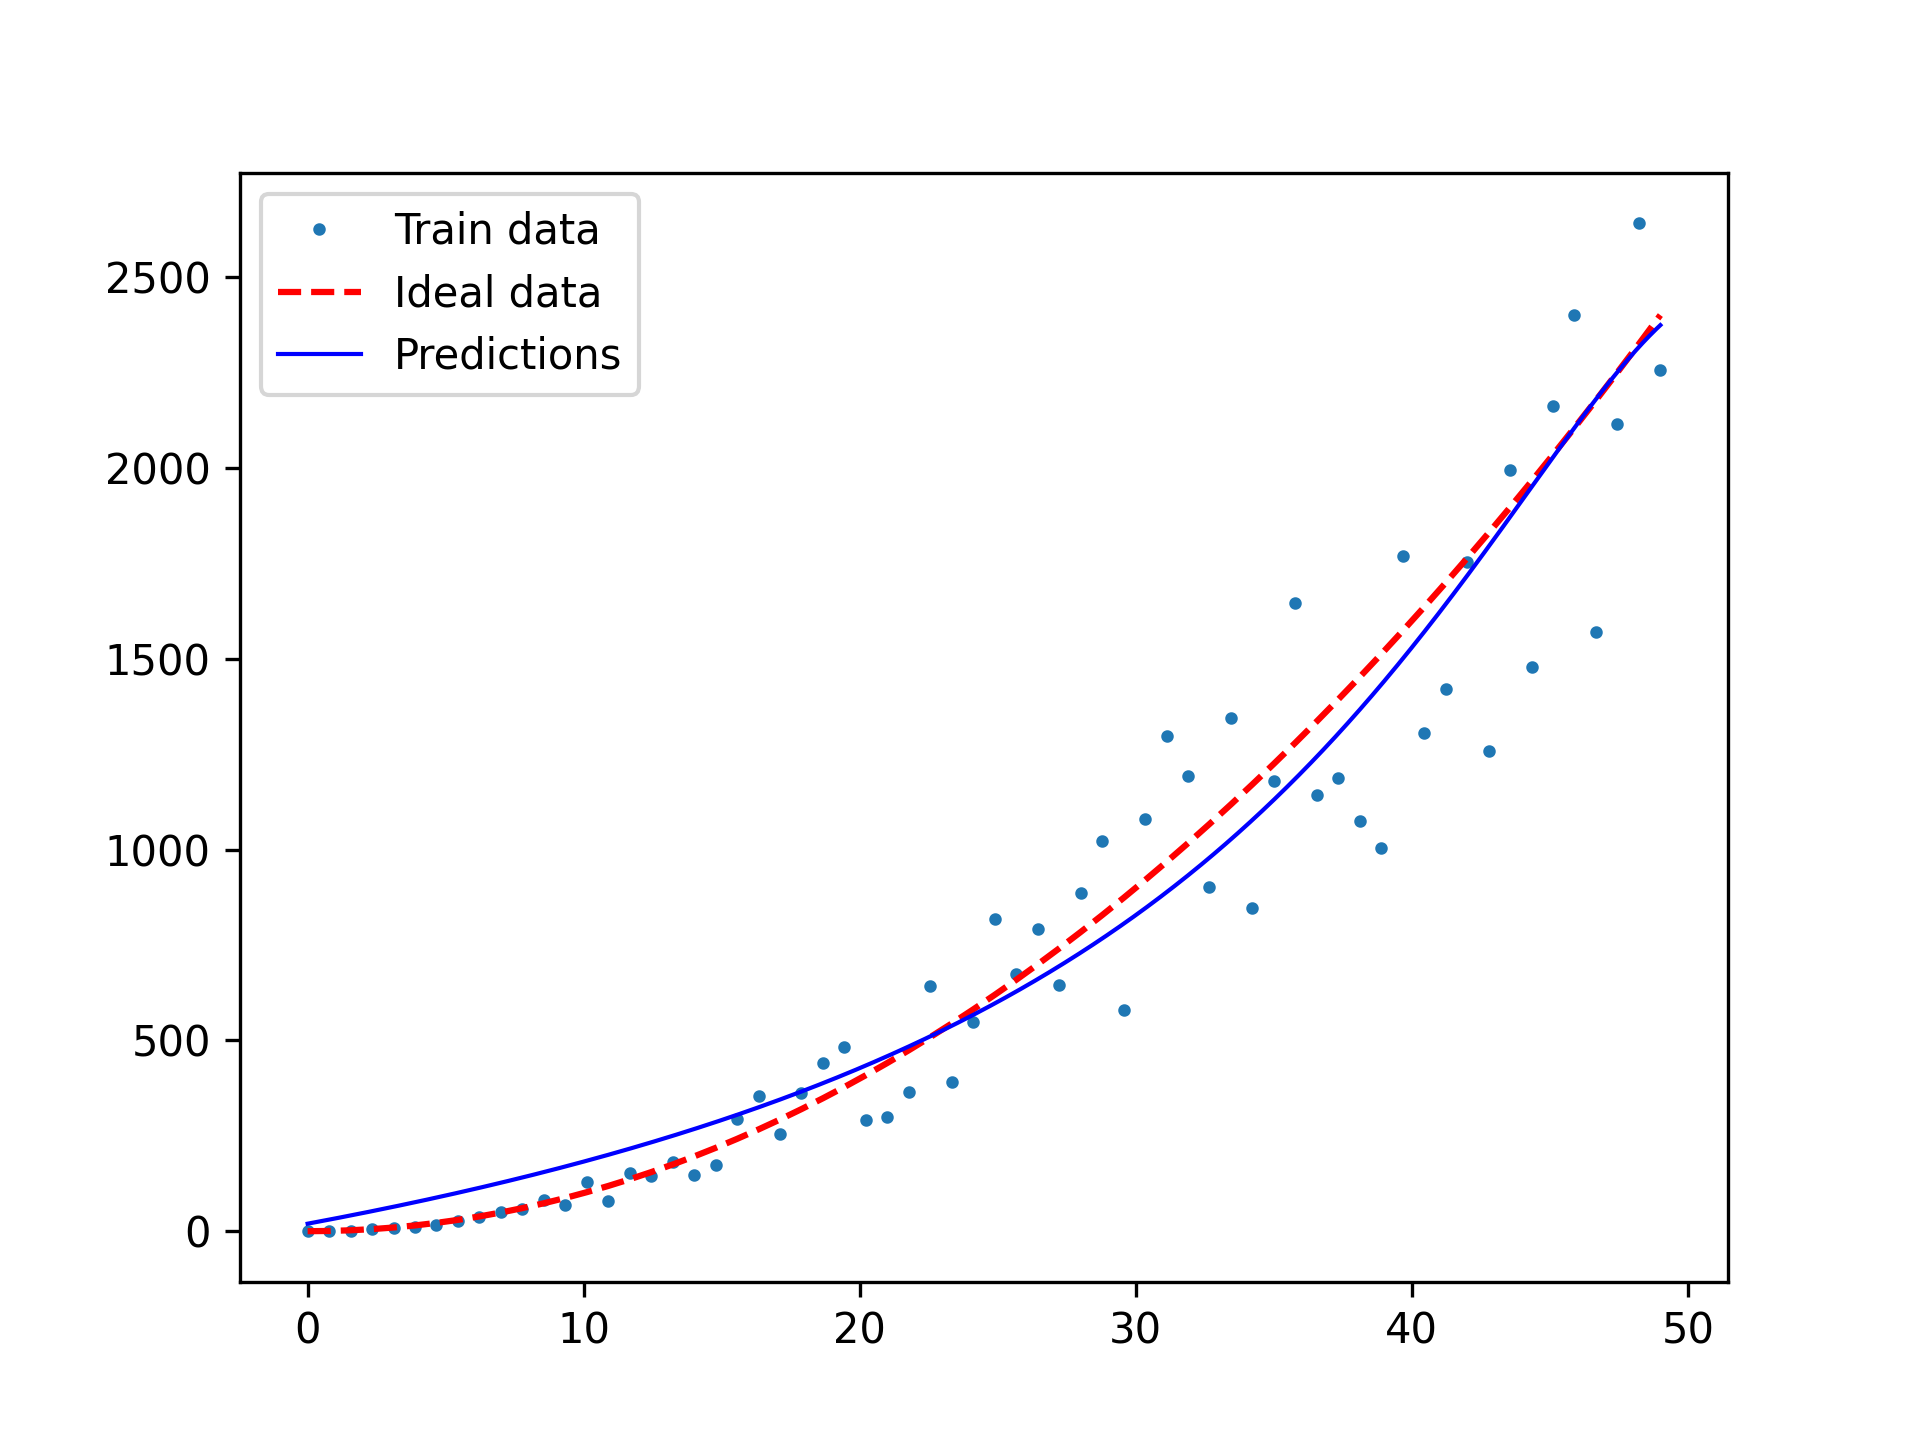
\includegraphics[width=0.5\textwidth]{./images/lambda.png}
    \caption{Gráfica de la selección de $\lambda$}
    \label{fig:seleccion_lambda_plot}
\end{figure}

\begin{figure}[H]
    \centering
    \lstinputlisting[firstline=147,lastline=166, style=custompython]{../design.py}
    \caption{Función \textit{train\_reg}}
    \label{fig:train_reg}
\end{figure}

\begin{figure}[H]
    \centering
    \lstinputlisting[firstline=264,lastline=307, style=custompython]{../design.py}
    \caption{Función \textit{seleccion\_lambda}}
    \label{fig:seleccion_lambda}
\end{figure}

\section{Elección de hiperparámetros}

En este apartado vamos a escoger grado y regularización mirando el mínimo coste de validación. Para ello usaremos los posibles parámetros de los dos apartados anteriores. La función \textit{seleccion\_hiperparametros} (figura \ref{fig:seleccion_hiperparametros}) nos ayudará a escoger el mejor grado y $\lambda$. La figura \ref{fig:seleccion_hiperparametros_plot} nos muestra la comparativa entre el modelo con los hiperparámetros escogidos y la recta ideal. Los hiperparámetros escogidos son grado 12 y $\lambda$ 1e-6.

Podemos ver los resultados por $\lambda$ (vertical) y grado (horizontal) en las tablas \ref{tab:hiper1} \ref{tab:hiper2} y \ref{tab:hiper3}.

\begin{figure}[H]
    \centering
    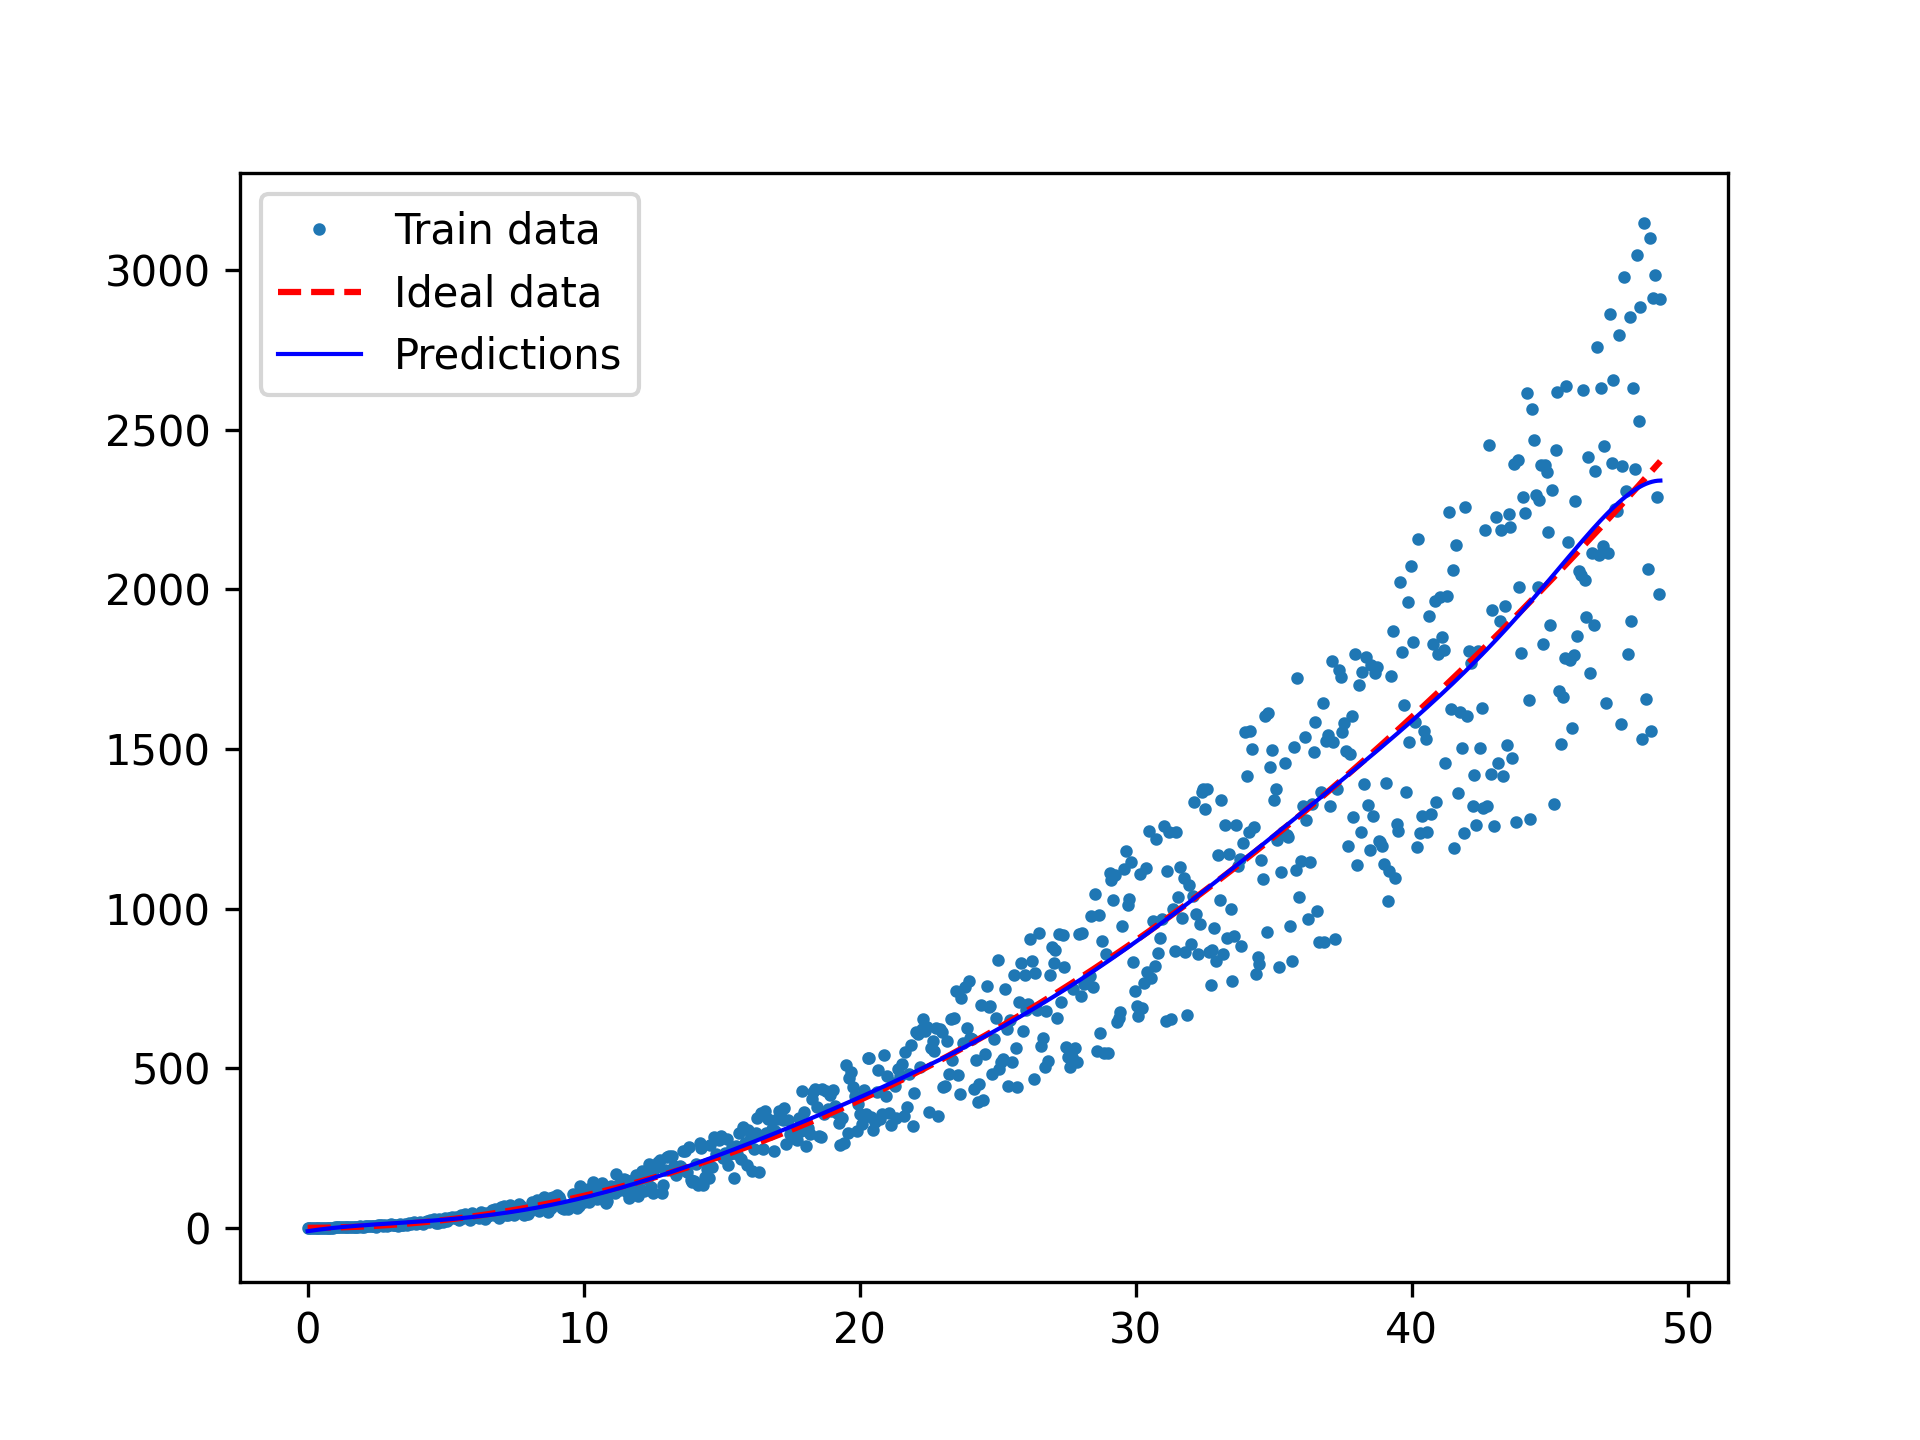
\includegraphics[width=0.5\textwidth]{./images/hiperparametros.png}
    \caption{Gráfica de la selección de hiperparámetros}
    \label{fig:seleccion_hiperparametros_plot}
\end{figure}

\begin{table}[H]
    \centering
    \csvautotabular{./csv/hiperparametros0.csv}
    \caption{Resultados de los hiperparámetros}
    \label{tab:hiper1}
\end{table}

\begin{table}[H]
    \centering
    \csvautotabular{./csv/hiperparametros1.csv}
    \caption{Resultados de los hiperparámetros}
    \label{tab:hiper2}
\end{table}

\begin{table}[H]
    \centering
    \csvautotabular{./csv/hiperparametros2.csv}
    \caption{Resultados de los hiperparámetros}
    \label{tab:hiper3}
\end{table}

\begin{figure}[H]
    \centering
    \lstinputlisting[firstline=310,lastline=370, style=custompython]{../design.py}
    \caption{Función \textit{seleccion\_hiperparametros}}
    \label{fig:seleccion_hiperparametros}
\end{figure}


\section{Curvas de aprendizaje}

En este apartado vamos a hacer una comparativa de coste de validación y de entrenamiento variando el tamaño de muestra de entrenamiento. Para ello usaremos la función \textit{learing\_curve} (figura \ref{fig:learning_curve}). La figura \ref{fig:curvas_aprendizaje_plot} nos muestra la comparativa entre el coste de validación y de entrenamiento. Para pintar la gráfica se ha usado la función \textit{draw\_learning\_curve} (figura \ref{fig:draw_learning_curve}).

\begin{figure}[H]
    \centering
    \includegraphics[width=0.5\textwidth]{./images/learning\_curve.png}
    \caption{Gráfica de las curvas de aprendizaje}
    \label{fig:curvas_aprendizaje_plot}
\end{figure}

\begin{figure}[H]
    \centering
    \lstinputlisting[firstline=373,lastline=400, style=custompython]{../design.py}
    \caption{Función \textit{learning\_curve}}
    \label{fig:learning_curve}
\end{figure}

\begin{figure}[H]
    \centering
    \lstinputlisting[firstline=58,lastline=71, style=custompython]{../design.py}
    \caption{Función \textit{draw\_learning\_curve}}
    \label{fig:draw_learning_curve}
\end{figure}


\section{Utilidades}

Algunas utilidades que se han usado en el código son las siguientes:
\begin{itemize}
    \item \textit{test\_overfitting} (figura \ref{fig:test_overfitting}): Función que testea el sobreajuste.
    \item \textit{test\_seleccion\_grado} (figura \ref{fig:test_seleccion_grado}): Función que testea la selección del grado.
    \item \textit{test\_regularización} (figura \ref{fig:test_regularizacion}): Función que testea la selección de $\lambda$.
    \item \textit{test\_hiperparametros} (figura \ref{fig:test_hiperparametros}): Función que testea la selección de hiperparámetros.
    \item \textit{test\_learning\_curve} (figura \ref{fig:test_learning_curve}): Función que testea las curvas de aprendizaje.
    \item \textit{write\_csv} (figura \ref{fig:write_csv}): Función que escribe los datos en un archivo \textit{csv}.
    \item \textit{main} (figura \ref{fig:main}): Función que ejecuta todas las pruebas.
    \item \textit{CommandLine} (figura \ref{fig:commandLine}): Clase que nos permite añadirle parámetros a la ejecución del programa.
\end{itemize}

\begin{figure}[H]
    \centering
    \lstinputlisting[firstline=403,lastline=422, style=custompython]{../design.py}
    \caption{Función \textit{test\_overfitting}}
    \label{fig:test_overfitting}
\end{figure}

\begin{figure}[H]
    \centering
    \lstinputlisting[firstline=425,lastline=437, style=custompython]{../design.py}
    \caption{Función \textit{test\_seleccion\_grado}}
    \label{fig:test_seleccion_grado}
\end{figure}

\begin{figure}[H]
    \centering
    \lstinputlisting[firstline=440,lastline=452, style=custompython]{../design.py}
    \caption{Función \textit{test\_regularizacion}}
    \label{fig:test_regularizacion}
\end{figure}

\begin{figure}[H]
    \centering
    \lstinputlisting[firstline=455,lastline=467, style=custompython]{../design.py}
    \caption{Función \textit{test\_hiperparametros}}
    \label{fig:test_hiperparametros}
\end{figure}

\begin{figure}[H]
    \centering
    \lstinputlisting[firstline=470,lastline=482, style=custompython]{../design.py}
    \caption{Función \textit{test\_learning\_curve}}
    \label{fig:test_learning_curve}
\end{figure}

\begin{figure}[H]
    \centering
    \lstinputlisting[firstline=74,lastline=89, style=custompython]{../design.py}
    \caption{Función \textit{write\_csv}}
    \label{fig:write_csv}
\end{figure}

\begin{figure}[H]
    \centering
    \lstinputlisting[firstline=492,lastline=508, style=custompython]{../design.py}
    \caption{Función \textit{main}}
    \label{fig:main}
\end{figure}


\begin{figure}[H]
    \centering
    \lstinputlisting[firstline=485,lastline=489, style=custompython]{../design.py}
    \caption{Función \textit{prepare\_folder}}
    \label{fig:prepare_folder}
\end{figure}

\begin{figure}[H]
    \centering
    \lstinputlisting[style=custompython]{../commandline.py}\caption{Clase \textit{CommandLine}}\label{fig:commandline}
\end{figure}

\end{document}
